\chapter{Mizuki Shigeru, GeGeGe no Kitarō and the Postwar Yōkai Boom}

\section{Mizuki Shigeru (1922--2015)}

If one person is responsible for the image of yōkai in contemporary Japan, it is the manga
artist \textbf{Mizuki Shigeru} (\ja{水木しげる}, real name Mura Shigeru).

\begin{center}
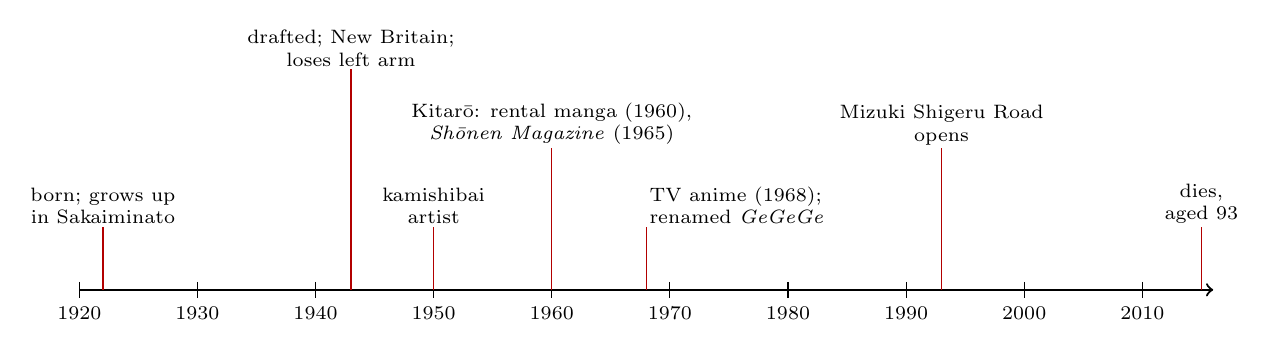
\begin{tikzpicture}[x=0.6cm, y=1cm, every node/.style={font=\scriptsize}]
  \draw[->, thick] (0,0) -- (24,0);
  \foreach \yr in {1920,1930,1940,1950,1960,1970,1980,1990,2000,2010} {
    \pgfmathsetmacro{\x}{(\yr-1920)/4}
    \draw (\x,0.1) -- (\x,-0.1) node[below] {\yr};
  }
  \foreach \yr/\lab/\h in {1922/{born; grows up\\in Sakaiminato}/0.8, 1943/{drafted; New Britain;\\loses left arm}/2.8,
      1950/{kamishibai\\artist}/0.8, 1960/{Kitarō: rental manga (1960),\\\emph{Shōnen Magazine} (1965)}/1.8,
      1993/{Mizuki Shigeru Road\\opens}/1.8, 2015/{dies,\\aged 93}/0.8} {
    \pgfmathsetmacro{\x}{(\yr-1920)/4}
    \draw[red!70!black] (\x,0) -- (\x,\h);
    \node[above, align=center, fill=white, inner sep=1pt] at (\x,\h) {\lab};
  }
  \draw[red!70!black] (12,0) -- (12,0.8);
  \node[above right, align=left, fill=white, inner sep=1pt] at (12,0.8) {TV anime (1968);\\renamed \emph{GeGeGe}};
\end{tikzpicture}
\end{center}

\subsection{Life}

\begin{itemize}
  \item \textbf{Childhood}: grew up in Sakaiminato, a port town in Tottori prefecture. An
        elderly woman who helped in the house, \textbf{Nonnonbā}, told him stories of yōkai
        and the other world. He later made her the subject of an autobiographical manga
        (\emph{Nonnonbā to ore}, 1977).
  \item \textbf{War}: drafted in 1943 and sent to Rabaul on New Britain (Papua New Guinea).
        Most of his unit was killed; he contracted malaria and lost his left arm in an air
        raid. He befriended local Tolai villagers and considered staying. His
        \emph{Onward Towards Our Noble Deaths} (\ja{総員玉砕せよ!}, 1973) is a
        largely autobiographical anti-war manga.
  \item \textbf{Postwar}: painted pictures for \emph{kamishibai} (paper theatre) street
        storytellers, then drew for the rental-book (\emph{kashihon}) manga market; poor
        until his forties.
  \item \textbf{Success}: from the mid-1960s, Kitarō and other works made him famous. He
        drew yōkai encyclopedias, a manga history of Shōwa Japan, and a biography of Hitler.
\end{itemize}

\begin{important}[War and yōkai]
Scholars and Mizuki himself linked his yōkai to his war experience. Yōkai represent a
world of spirits, nature and the dead that modern, militarized, then economically driven
Japan had tried to destroy. His humour and his insistence on ``taking it easy'' (he
admired the relaxed life of the Tolai) are a critique of the regimented society that sent
his comrades to die.
\end{important}

\section{GeGeGe no Kitarō}

\subsection{Origins}

Kitarō began in a 1930s kamishibai tale, \emph{Hakaba Kitarō} (``Graveyard Kitarō''), which
Mizuki adapted in his rental manga around 1960. Early Kitarō was a creepy, amoral boy born
in a grave. When the series moved to \emph{Weekly Shōnen Magazine} (1965) and to TV anime
(1968), it was renamed \emph{GeGeGe no Kitarō} (\ja{ゲゲゲの鬼太郎}) and Kitarō became a
hero who protects humans from bad yōkai. (``GeGeGe'' comes from Mizuki's childhood
nickname, from his mispronunciation of his own name.)

\subsection{Characters}

\begin{center}
\begin{tabular}{llp{8.5cm}}
\toprule
Character & Japanese & Description \\
\midrule
Kitarō & \ja{鬼太郎} & one-eyed yōkai boy (hair covers the empty socket), last of the ghost tribe; striped vest, wooden geta; hair needles, remote-controlled geta \\
Medama-oyaji & \ja{目玉おやじ} & ``Eyeball Father'': his dead father, reborn as an eyeball with a tiny body; bathes in a teacup \\
Nezumi-otoko & \ja{ねずみ男} & ``Rat Man'': half-human half-yōkai, greedy, smelly, untrustworthy; Kitarō's frenemy \\
Neko-musume & \ja{猫娘} & ``Cat Girl'': turns into a fanged cat when angry \\
Sunakake-babā & \ja{砂かけ婆} & sand-throwing old woman \\
Konaki-jijī & \ja{子泣き爺} & old man who cries like a baby and becomes heavy as stone \\
Ittan-momen & \ja{一反木綿} & a flying strip of cotton cloth, used as transport \\
Nurikabe & \ja{ぬりかべ} & an invisible wall that blocks the road at night; drawn as a big, mild-faced wall \\
\bottomrule
\end{tabular}
\end{center}

\begin{center}
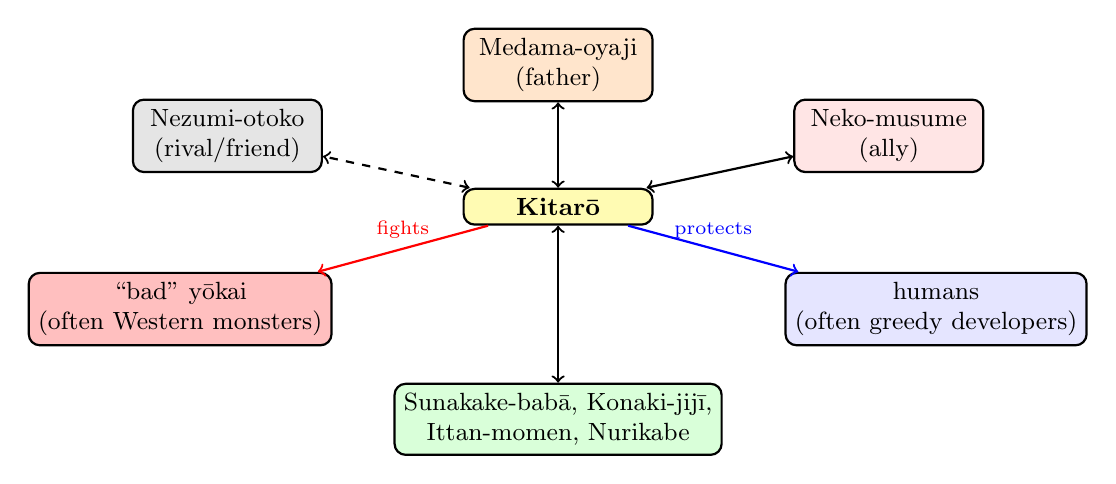
\begin{tikzpicture}[b/.style={draw, thick, rounded corners, align=center, font=\small, minimum width=2.4cm}]
  \node[b, fill=yellow!30] (k) at (0,0) {\textbf{Kitarō}};
  \node[b, fill=orange!20] (m) at (0,1.8) {Medama-oyaji\\(father)};
  \node[b, fill=gray!20] (n) at (-4.2,0.9) {Nezumi-otoko\\(rival/friend)};
  \node[b, fill=pink!40] (c) at (4.2,0.9) {Neko-musume\\(ally)};
  \node[b, fill=green!15] (allies) at (0,-2.7) {Sunakake-babā, Konaki-jijī,\\Ittan-momen, Nurikabe};
  \node[b, fill=red!25] (bad) at (-4.8,-1.3) {``bad'' yōkai\\(often Western monsters)};
  \node[b, fill=blue!10] (hum) at (4.8,-1.3) {humans\\(often greedy developers)};
  \draw[<->, thick] (k) -- (m);
  \draw[<->, thick, dashed] (k) -- (n);
  \draw[<->, thick] (k) -- (c);
  \draw[<->, thick] (k) -- (allies);
  \draw[->, thick, red] (k) -- node[above, font=\scriptsize] {fights} (bad);
  \draw[->, thick, blue] (k) -- node[above, font=\scriptsize] {protects} (hum);
\end{tikzpicture}
\end{center}

\begin{example}[Yōkai vs.\ Western monsters]
In a famous storyline, Kitarō battles a ``Yōkai Great War'' against invading Western
monsters (Dracula, a witch, Frankenstein's monster, a werewolf). Japanese yōkai are
defenders of home ground against foreign monsters, which can be read as a postwar
allegory about American cultural power, though the tone is comic.
\end{example}

\subsection{Six (and counting) anime series}

The anime has been remade roughly once per decade (1968, 1971, 1985, 1996, 2007, 2018),
each reflecting its time: the 1985 version during the bubble economy, the 2018 version
dealing with social media and urban loneliness. Each remake produced a new ``yōkai boom''
among children.

\section{Mizuki as encyclopedist}

Mizuki drew hundreds of yōkai in encyclopedias and field-guide formats (e.g.\ \emph{Nihon
yōkai taizen}). He relied heavily on Toriyama Sekien and on Yanagita's \emph{Yōkai dangen}:

\begin{itemize}
  \item He gave visual form to yōkai that Yanagita had recorded only as names. For
        example, \emph{nurikabe} in Yanagita is a phenomenon (an invisible wall you
        meet on a night road in Kyushu); Mizuki drew it as a creature.
  \item He invented or embellished many details, which are now accepted as ``tradition''.
  \item His art style mixed cartoony characters with very detailed, realistic, dark
        backgrounds (often traced from photographs), producing the uncanny feeling that
        yōkai inhabit the real world.
\end{itemize}

\begin{center}
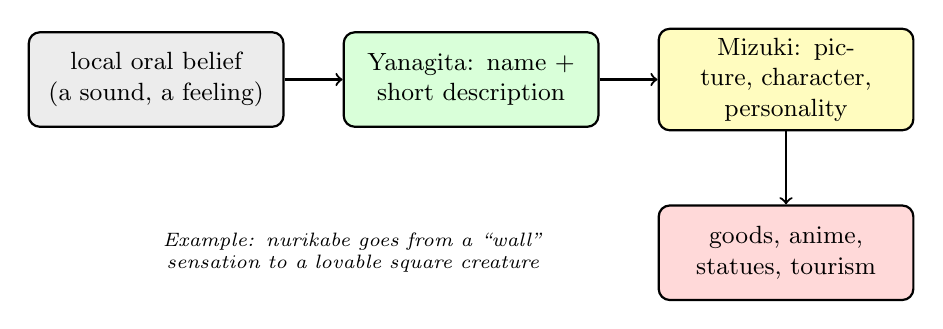
\begin{tikzpicture}[b/.style={draw, thick, rounded corners, align=center, font=\small, text width=3cm, minimum height=1.2cm}]
  \node[b, fill=gray!15] (oral) at (0,0) {local oral belief\\(a sound, a feeling)};
  \node[b, fill=green!15] (yan) at (4,0) {Yanagita: name + short description};
  \node[b, fill=yellow!25] (miz) at (8,0) {Mizuki: picture, character, personality};
  \node[b, fill=red!15] (pop) at (8,-2.2) {goods, anime, statues, tourism};
  \draw[->, thick] (oral) -- (yan); \draw[->, thick] (yan) -- (miz); \draw[->, thick] (miz) -- (pop);
  \node[font=\scriptsize\itshape, text width=6cm, align=center] at (2.5,-2.2) {Example: nurikabe goes from a ``wall'' sensation to a lovable square creature};
\end{tikzpicture}
\end{center}

\section{The yōkai boom and its meaning}

\begin{itemize}
  \item The late 1960s boom coincided with the costs of high-speed growth: environmental
        pollution (Minamata disease) and the loss of the countryside, producing nostalgia for disappearing rural life. Yōkai
        stood for nature and the past.
  \item Foster connects yōkai to Japan's \emph{furusato} (``old home village'') nostalgia
        and to the ``disappearing'' of the countryside.
  \item \textbf{Sakaiminato}: since 1993 the ``Mizuki Shigeru Road'' has over 150 bronze
        yōkai statues and a museum. It turned a declining fishing town into a major tourist
        destination, especially after the 2010 NHK drama \emph{GeGeGe no Nyōbō} about
        Mizuki's wife.
  \item The novelist Kyōgoku Natsuhiko (\emph{The Summer of the Ubume}, 1994) and the
        World Yōkai Association continued Mizuki's project in the 1990s.
\end{itemize}

\begin{aside}
Mizuki's ``Seven Rules for Happiness'' sum up his outlook. Two of them: ``Do what you
find fun, not what you think will succeed'' and ``Believe in the invisible world.''
\end{aside}

\section*{Summary}
\begin{itemize}
  \item Mizuki Shigeru: childhood yōkai stories (Nonnonbā), war in New Guinea, poverty,
        then fame from the 1960s.
  \item \emph{GeGeGe no Kitarō}: from creepy graveyard boy (c.\ 1960) to heroic yōkai protector
        (1965 manga, 1968 anime); remade every decade.
  \item Mizuki's encyclopedias gave form to yōkai known only by name; much ``tradition''
        is his invention.
  \item The postwar yōkai boom expresses nostalgia and critique of modernization; it
        revitalized Sakaiminato through tourism.
\end{itemize}
